

    %(Fill in bits about the squeezer)

Gravitational wave interferometry measures changes in light travel time far less than the light-crossing time of an atom, so the quantum nature of light has always influenced detector design.
Advanced LIGO aims to resolve most of noise sources described in Sections~\ref{methods} and~\ref{interferometer_theory}: even so, quantum shot and radiation pressure noise from light will remain.
Carlton Caves correctly derived the quantum behavior of interferometer shot and radiation pressure noise~\cite{Caves1980}.
Prior work had inferred the shot noise level from classical principles, accurately, but been ambiguous about radiation pressure.
With the quantum noise clarified, it was realized that this noise could be reduced through so-called squeezing of the vacuum state~\cite{Caves1981}.
This chapter describes part of how squeezing was successfully realized three decades later at the LIGO Hanford Observatory.
For additional details, consult Chua~\cite{ChuaThesis} and Dwyer~\cite{DwyerThesis}.

    \section{Squeezing theory}
    \label{squeezing_theory}

      %  Squeezing theory.
Quantum noise was initially treated as Poissonian photon counting (shot noise) and momentum coupling (radiation pressure), but it is better understood as the phase and amplitude uncertainty of the electromagnetic field at the interferometer output. 
Roughly speaking, phase uncertainty is equivalent to semi-classical shot noise and amplitude uncertainty to radiation pressure.
The standard quantum limit (SQL) on displacement sensitivity can be derived independently of either argument, as noted by Caves~\cite{Caves1981}:

\begin{equation}
(\Delta z)_{\textup{SQL}} = (2 \hbar \tau / m)^{1/2},
\label{sql_caves}
\end{equation}

\noindent where in Equation~\ref{sql_caves} $z$ is the mirror (test mass) displacement, $\tau$ is measurement duration, $\hbar$ is the reduced Planck constant, and $m$ is mirror mass.
When one tries to attain this standard quantum limit with an interferometer, then shot and radiation pressure are found to balance at a particular optimum input power $P_0$~\cite{Caves1981}:

\begin{equation}
P_0 = \frac{1}{2} \frac{mc^2}{\tau}\frac{1}{\omega \tau} \frac{1}{b^2} \equiv {\hbar \omega \alpha_0^2}{\tau},
\label{optimum_power_caves}
\end{equation}

\noindent with $\omega$ the angular frequency of light and $b$ the number of bounces (assuming delay lines, whereas a Fabry-Perot is proportional to finesse) in Equation~\ref{optimum_power_caves} and $\alpha_0 = \sqrt{P \tau / \hbar \omega}$ is the number of photons.
The latter equation shows that the optimal power rises as $1/\sqrt{\tau}$, that is, as the squart root of the gravitational wave frequency.
Higher laser power improves high frequency sensitivity, high mirror mass improves low frequency performance.
Combined, these formulae imply that an interferometer should be built with the largest, most massive mirrors and most powerful lasers practicable.

        \subsection{Problems with lasers: thermal compensation}
        \label{TCS}

            %Experience (some firsthand) with thermal compensation.

LIGO and its allied interferometers do try to operate with massive optics and powerful lasers, but there are limits.
Vacuum enclosures place a constraint, only broken with significant expenditures, on the size of optical tables and mirror suspensions and therefore on mirror mass.
This indirectly limits laser power through the SQL.
Laser power, however, was not limited for this reason in initial and enhanced LIGO.
In practice, thermal distortion of the test masses was a worse problem~\cite{BallmerThesis}.
Absorption, both in the bulk of the fused silica substrate and in the HR coatings, of a few parts per million was sufficient to distort the radius of curvature of the Fabry-Perot cavities.
While managed with a $\textup{CO}_2$ laser-driven thermal compensation system (supplemented with ring heaters in aLIGO), this thermal distortion remains a serious concern.

Having an alternative to increased mirror size and laser power would grant flexibility.
Hence squeezing: the standard quantum limit can be achieved through another means.


        \subsection{Quantum shot noise and radiation pressure}
        \label{quantum_noise}

            %Carlton Caves, quantum shot noise and radiation pressure.

%\begin{frame}{Squeezing introduction}

%\begin{definition}

Squeezing as used in the context of gravitational made interferometer has a specific meaning.
While no alterations are made to the input laser light, the output `dark' port of the interferometer, whence comes the light received by the photodetector, is changed.
The output port in a squeezed interferometer receives a squeezed vacuum state from the opposite direction to the laser light.
This squeezed vacuum state is prepared on a `squeezer' table.
This beam is injected with the correct polarization, using a Faraday isolator and wave plates to guard against laser light entering the squeezer, and propagates through the interferometer arms (requiring proper alignment) until it and the laser light are both incident on the same output photodetector.
The desired effect is altering $\Delta E\Delta\phi$ uncertainty for the vacuum state of the electromagnetic field.
Reducing $\Delta \phi$ at the cost of still-acceptable $\Delta E$ permits\footnote{$\Delta E$ can also be squeezed; see Section~\ref{third-gen_squeezing}} a more precise measurement, equivalent to the beneficial effect of increasing laser power but without heating the mirrors.
Casually, more laser power boosts the shot-noise limited `signal' of a high-frequency measurement whereas squeezing reduces the `noise'. 
Formally, the expectation value of quantum operators is improved.

%\begin{theorem}
%Shot noise arises from quantum operators (Caves 1980, 1981)\end{theorem}

Caves's prescription~\cite{Caves1981} is clear:
\begin{itemize}
\item Vacuum fluctuations couple through anti-symmetric port, so inject a
\item \emph{Squeezed } $\overrightarrow{E}$ field (uncertainty ellipse with smaller $\Delta E$) defined by
\item Squeeze operator $S$ in Equation~\ref{squeeze_operator_caves} (with squeeze angle $\theta$, factor $r$, creation operator $a$):
\end{itemize}
%From the Caves squeezing paper~\cite{Caves1981},

\begin{equation}
S(\zeta)=\exp[\frac{1}{2}\zeta^{*}a^{2}-\frac{1}{2}\zeta(a^{\dagger})^{2}],\;\zeta=re^{i\theta}
\label{squeeze_operator_caves}
\end{equation}

\noindent thereby reducing shot noise by a factor of $e^{-r}$. The optimum power changes accordingly: Caves shows that $P_\textup{opt} = P_0 e^{-2r}$, so long as $|\alpha|\gg\sinh^2r$ and $|\alpha|\gg e^{2r}\sinh^2 r$. 

For a 20 W interferometer using 1.064 nm to measure at 100 Hz, the latter squeezing condition would be an issue around $r\geq10$, but to reduce optimal power by $1/2$ only requires $r \approx 0.34$. 
Trying to reduce optimal power by orders of magnitude is unlikely to occur any time soon: rather, a modest laser as would ordinarily be used in an interferometer can be supplemented with a squeezed beam to increase its effective power. 
Squeezing is an addition, not a replacement.
Yet the squeeze beam still must be physically generated, and this along with optical losses in the interferometer prove a much more significant challenge than theoretical constraints.

%Squeezed state made with
%optical parameter oscillator, 2nd harmonic generator
Squeezing can be physically generated through the use of an optical parametric oscillator (OPO).
Optical parameteric amplifiers, including an OPO, involve a nonlinear optical medium that is pumped with an electromagnetic wave at $\omega_p$.
An OPO~\cite{Caves1981} is an optical parametric amplifier for which the output `signal' (at $\omega_s$) and `idler' (at $\omega_i$) beams\footnote{The nomenclature is historical, sometimes distinguished by $\omega_s\geq\omega_i$. After alignment is complete, the output beams contain no power by design.} are degenerate (for any amplifier they satisfy $\omega_s + \omega_i$ = $\omega_p$, the input, pump frequency).
As Takahashi noted~\cite{Takahashi1965} (and others, see Wall for a review~\cite{Walls1983}), a degenerate amplifier will transform a coherent state into a state with unequal uncertainties in its two quadratures, to wit, phase and amplitude.

By placing a degenerate amplifier in cavity resonant at $\omega_s$, the amplifier becomes an optical parameter \textit{oscillator}, with high effective interaction length and thus squeeze factor.
Nonlinear media come in many varieties, but the material used in LIGO squeezing experiments (as in this chapter) has typically been PPKTP (periodically-poled potassium titanyl phosphate).
For an effective second-order nonlinear susceptability $d$, pump electric field amplitude $E_p$, effective interaction length $L$, and index of refraction at the signal frequency $n_s$, the amount of squeezing is~\cite{Caves1981},

\begin{equation}
r = \left(\frac{4\pi \omega_s L}{c n_s} \right) d |E_p|.
\label{how_much_squeezing}
\end{equation} 

\noindent Another, heuristic\footnote{Popularized by Daniel Sigg, formally described as sidebands in Dwyer~\cite{DwyerThesis}.}, understanding of the OPO (when $\omega_p = 2\omega)$ is that a vacuum fluctuation $\epsilon$ at $A e^{i\omega_\epsilon t + \phi_\epsilon}$ couples to the pump and so induces a second beam at amplitude $A e^{i\left(2\omega - (\omega_\epsilon t + \phi_\epsilon)\right)}$.
The superposition of these two beams has amplitude $\approx 2 A$ but phase $\approx (\phi_\epsilon - \phi_\epsilon)$, \textit{i.e.}, the ampltitude fluctuations (radiation pressure) have increased but the phase fluctuations (shot noise) have been reduced.

One caveat: the pump must be phase matched to the main laser (at $\omega$) of the overall interferometer.
This is usually accomplished (as at the Hanford experiment) with a small beamsplitter siphoning a portion of the laser (then, at Hanford, through a polarization-preserving fiber) and directing it to a second harmonic generator (SHG), which yielded $\omega_p = 2\omega$.
SHGs themselves operate using non-linear crystals to frequency-double incident laser light.
Imperfect phase matching is one of two chief reasons why squeezing can underperform.

The other reason for degraded squeezing is optical losses.
These can include absorption, scattering, and imperfect mode-matching.
While beyond the scope of this chapter, these optical losses are the principle reason that interferometer squeezing at the H1 photodetector in our experiment was about half what was generated in the OPO and must be addressed as squeezed light sources become more widespread.

Demonstrated first at GEO600~\cite{GEO600NatureSqueezing} then on H1 at the LIGO Hanford Observatory~\cite{BarsottiNatureSqueezing}, squeezing is now a proven technique.
At Hanford, the subject of this chapter, 2.15 dB of squeezing (28\%, equivalent to a 64\% increase in laser power~\cite{BarsottiNatureSqueezing}) was achieved with the combined efforts of Sheila Dwyer, Sheon Chua, Lisa Barsotti, Matt Evans, Keita Kawabe, Daniel Sigg, Conor Mow-Lowry, Alexander Khalaidovski, Maxim Factourovich, Nicol\'{a}s Smith-Lefebvre, Robert Schofield, Mike Landry, Cheryl Vorvick, and Richard Gustafson.
A picture of the squeezer and some of its scientists is shown in Figure~\ref{squeezing_team_pictured}.
The squeezing experiment was well-received by the entire staff\footnote{Quite busy themselves with Advanced LIGO installation.} of Hanford Observatory, to whom the squeezers were grateful.
This success encourages development of a production-quality squeezed light source for a future upgrade to Advanced LIGO, along the lines of Section~\ref{third-gen_squeezing}.
Squeezed light should increase aLIGO's performance and could prove critical to its successors, especially should they operate at cryogenic temperatures.

\begin{figure}
\begin{center}
%\protect\caption{\protect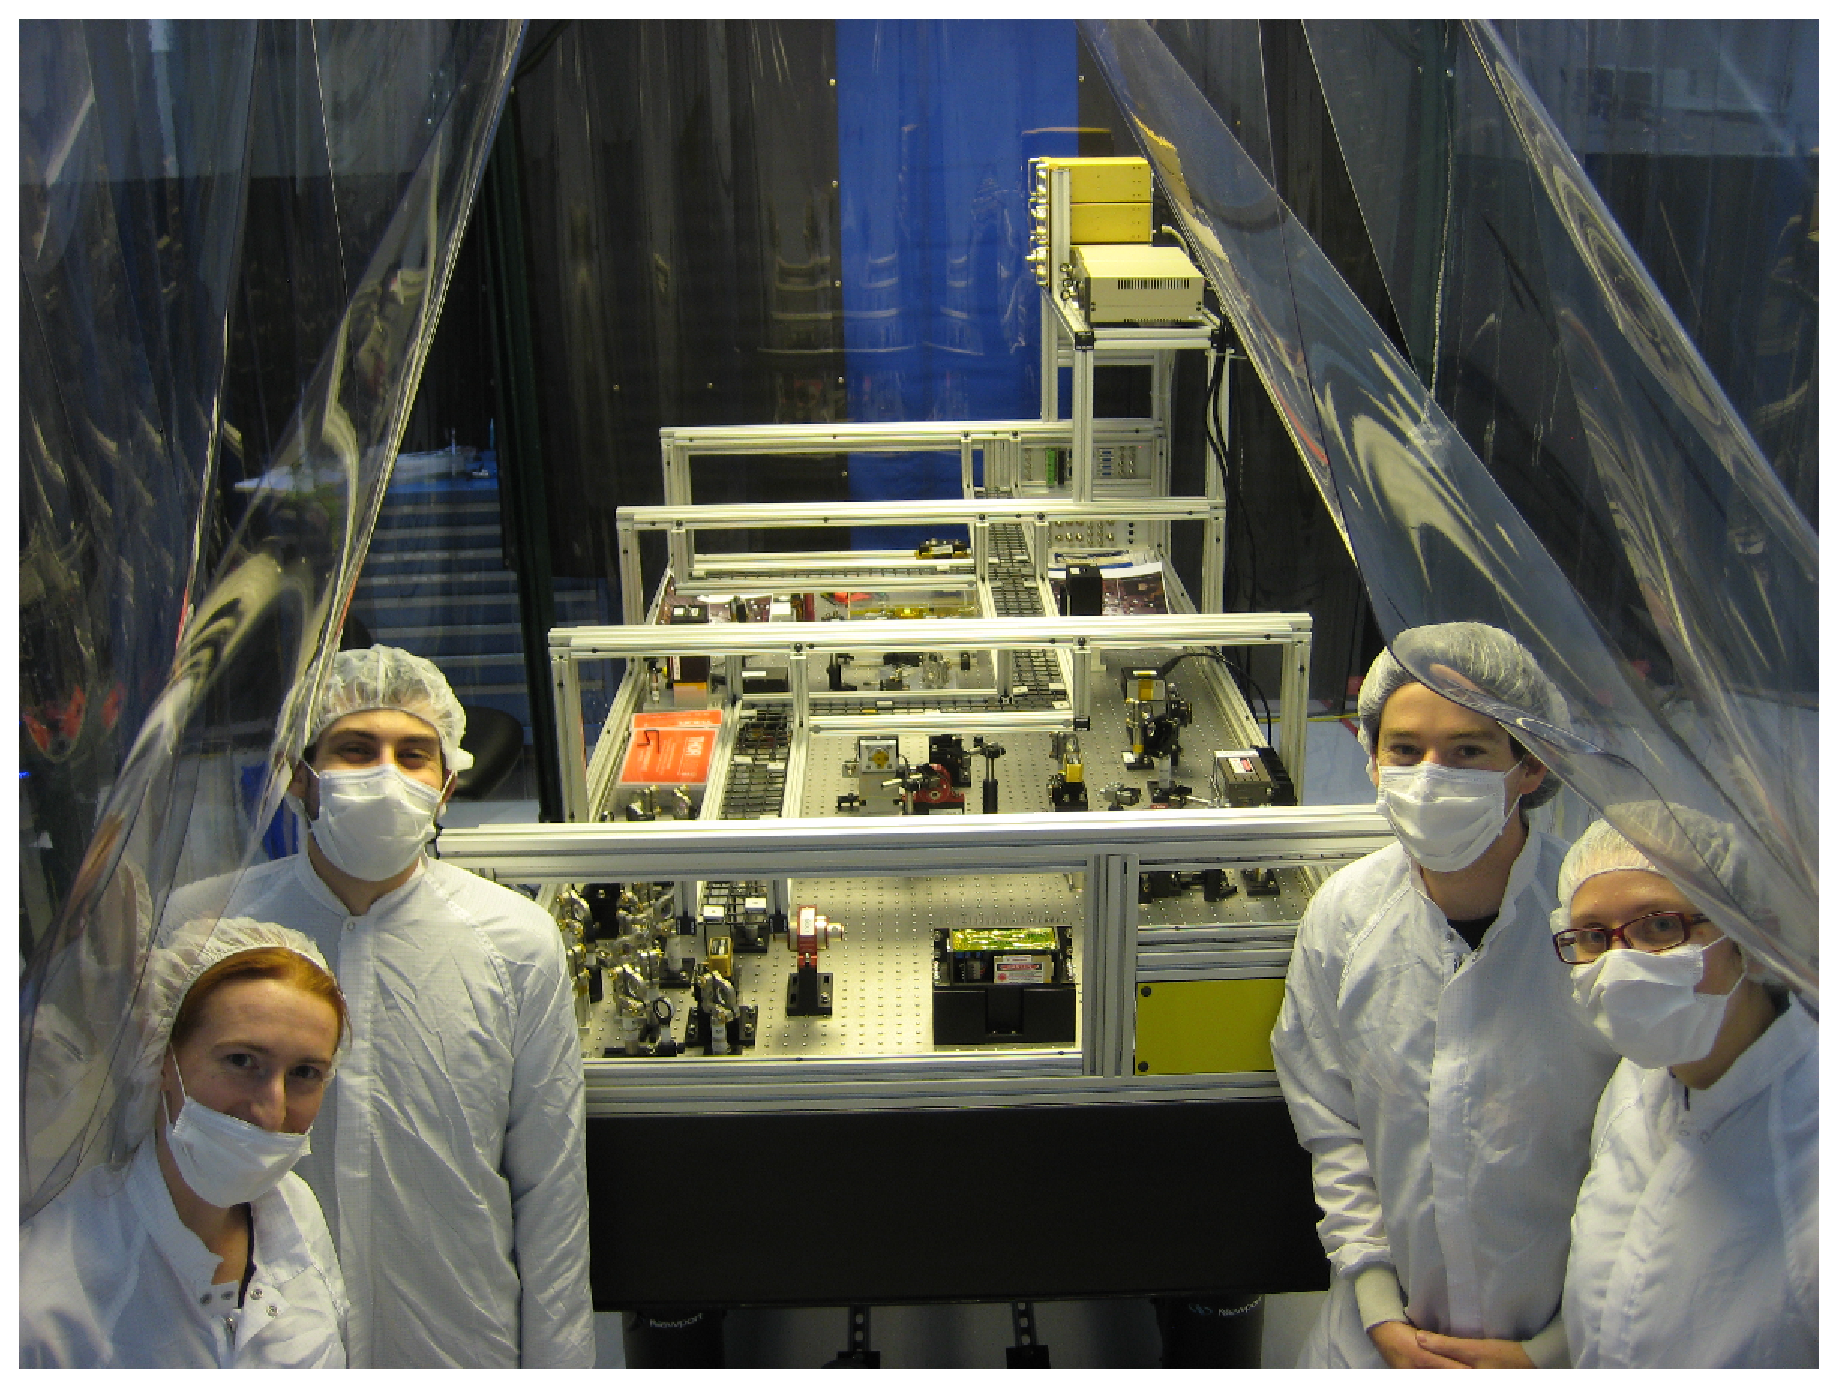
\includegraphics[width=0.33\paperwidth]{lisabar-1289966130}}
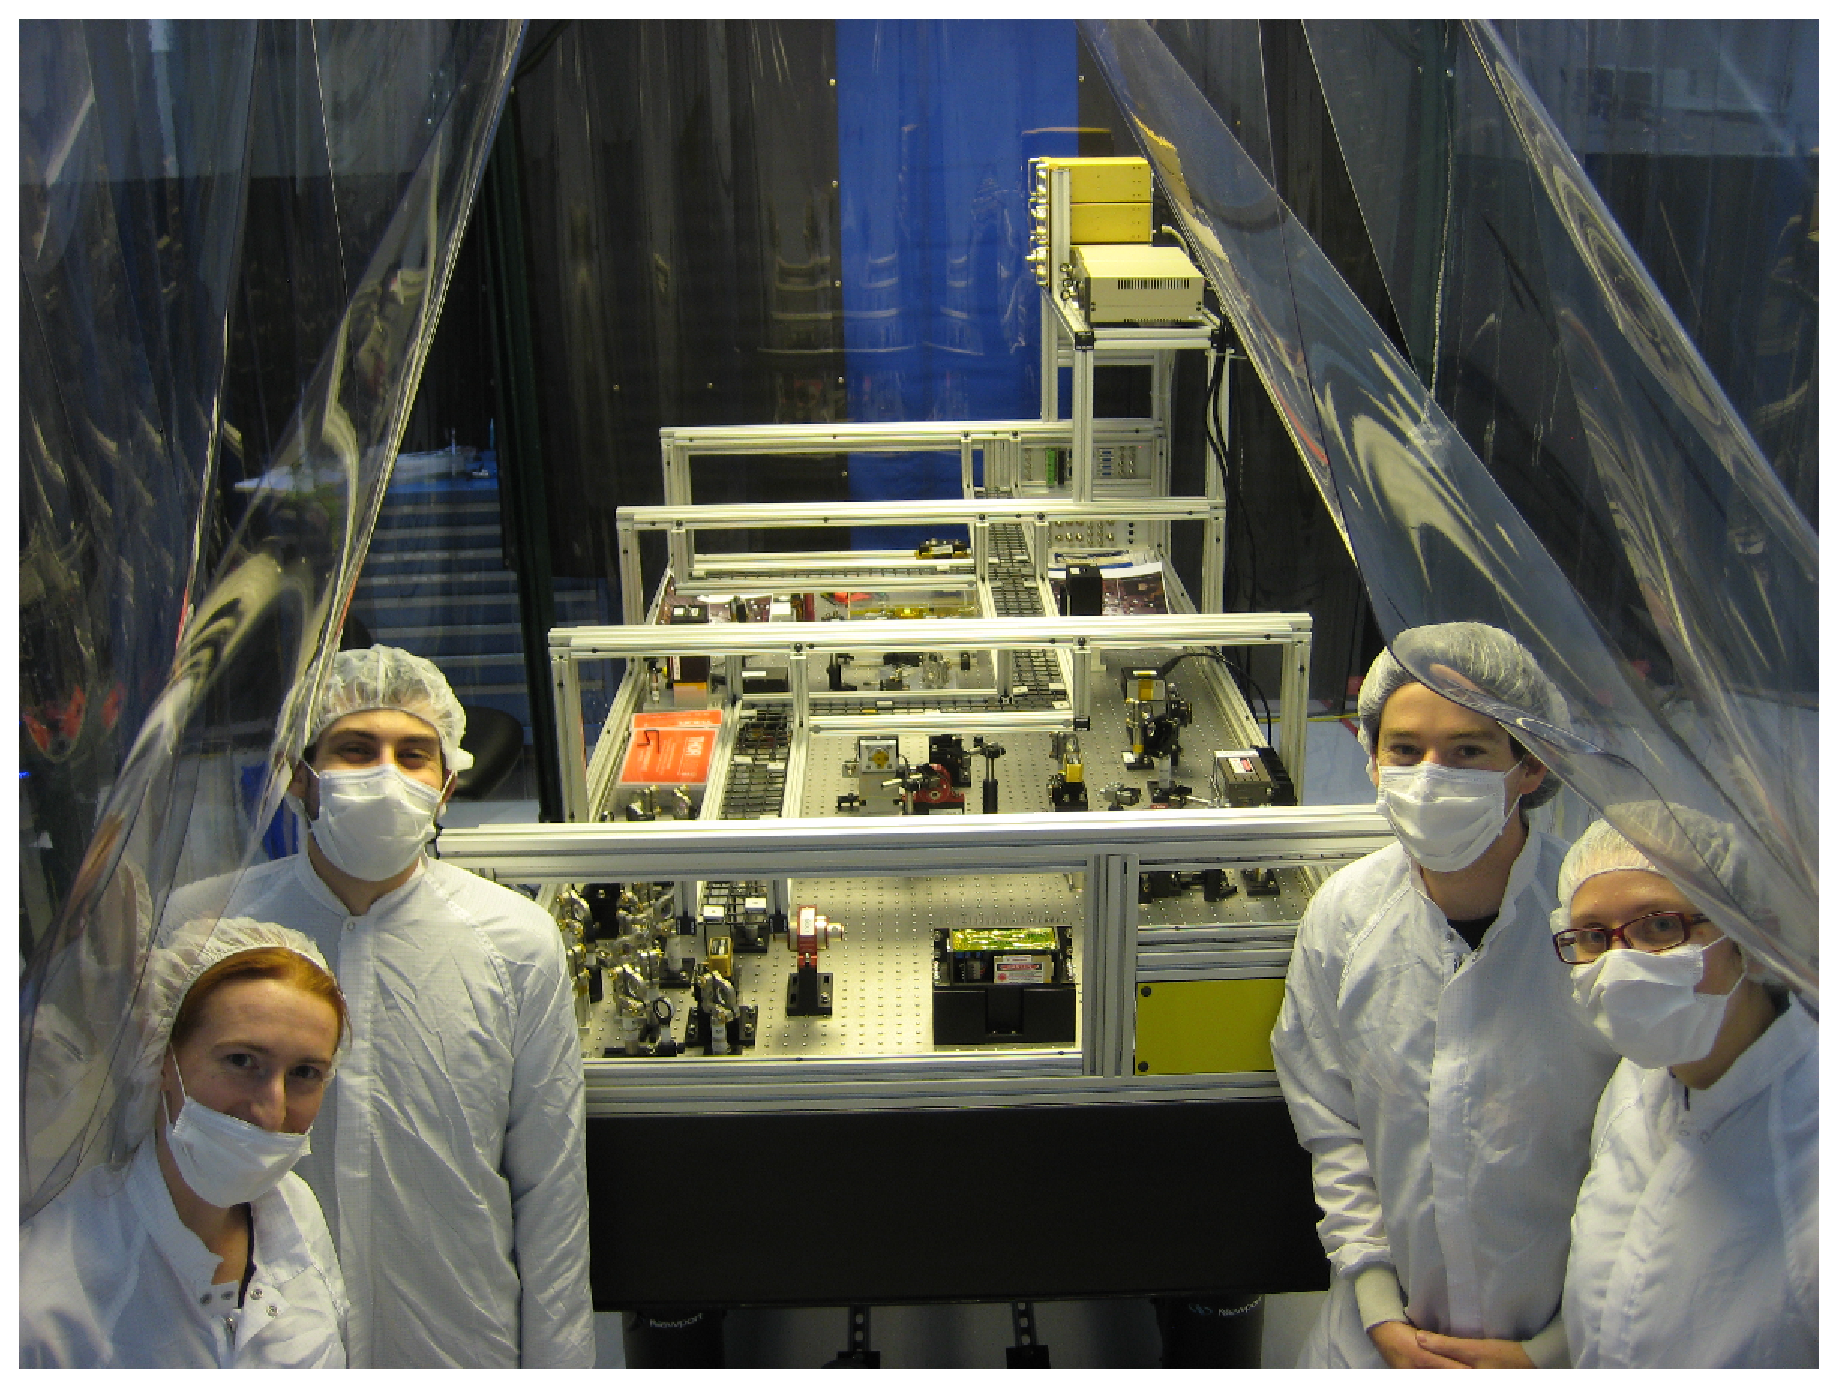
\includegraphics[width=0.6\paperwidth]{lisabar-1289966130.eps}
%\protect\caption{\protect\includegraphics[width=0.33\paperwidth]{lisabar-1300943141}}
\caption{Image by Lisa Barsotti in Hanford eLog.
\newline Counterclockise from lower left: Sheila Dwyer, Lisa Barsotti, Conor Mow-Lowry, Grant Meadors. This photograph shows the uncovered squeezer table with components from the MIT squeezer experiment unpacked at LIGO Hanford Observatory in November 2010. The table sat in a temporary location by HAM6, where it was recommissioned by Dwyer, Mow-Lowry, Sheon Chua, and Alexander Khalaidovksi until H1 could be brought back online for the squeezing experiment in late 2011. 
}
\label{squeezing_team_pictured}
\end{center}
\end{figure}



%\end{definition}
%\begin{itemize}
%\item Demonstrated first at GEO 600, then LIGO Hanford (H1)\end{itemize}

        \subsection{Squeezing filter cavities}
        \label{third-gen_squeezing}

Future squeezed light sources may prove more sophisticated still.
Equation~\ref{squeeze_operator_caves} includes an angle $\omega$. When $\zeta$ is positive, squeezing is generated and phase fluctuations diminish, as discussed above. 
The converse, $\zeta$ negative, yields anti-squeezing, where amplitude fluctuations are smaller. 
This angle $\omega$ is controlled by adjusting the phase of the main laser pickoff as it enters the OPO.
It would be benefical if amplitude fluctuations could be reduced at the frequencies where they are the dominant noise sources and likewise simultaneously with phase fluctuations. 
Such simultaneously reduction can in principle be accomplished with a filter cavity, which can rotate the squeezing uncertainty ellipse in a frequency-dependent way, as Chua summarizes~\cite{ChuaThesis}.
Prototypes at gravitational wave interferometer frequencies are under construction.
If promising, they might be tested at the observatories in a few years time.

    \section{LIGO Hanford Observatory quantum vacuum squeezing}
    \label{LHO_squeeze}

 %       Quantum vacuum squeezing at LIGO Hanford Observatory. 
%Naturally, a great deal of description and background will come from Sheila Dwyer's thesis~\cite{DwyerThesis} and Sheon Chua's thesis~\cite{ChuaThesis}.

        \subsection{Collaboration and contributions}
        \label{contributions}

        Squeezing tests at LIGO Hanford Observatory had been planned for several years in advance.
Nergis Malvalvala at the Massachusetts Institute of Technology, David McClelland at Australian National University, and Daniel Sigg at Hanford made arrangements for a prototype squeezer to be developed at MIT, with an OPO developed by ANU.
Experience with squeezing at GEO600 (Roman Schnabel and Henning Vahlbruch) informed planning. 
When the prototype squeezer had been made functional at MIT, it was disassembled and shipped cross-country to LHO.
There it was reassembled and integrated into the 4-kilometer interferometer by a team led by Barsotti, Sigg, and Kawabe, with Dwyer and Chua in charge of optics and operation.
This author's contributions were comparatively minor: the design and installation of supports for the optical table, assistance with in-vacuum installation and measurements of both optics and electronics, as well as interpretation of the squeezing results in astrophysical significance.

            %Contributions: table, in-vacuum installation, electronics, range est.

            \subsubsection{Optical table support assembly}
            \label{table_legs}

No space for an entire squeezing table or the constituent optics as then laid out existed inside the H1 vacuum enclosure.
Thus a new location had to be found, situated close to the beam splitter's dark port.
This site was by the vacuum chamber known as HAM4.
HAM4 had a free viewport, initially covered by steel then provided a vacuum window by Vorvick and Gerardo Moreno, wherein the squeezed light beam could be injected toward the dark port.
While the optics were installed and aligned on a spare, standard optical table, additional support for the table needed to be manufactured.
Existing prototype legs for the table were incorporated due to their good theoretical isolation performance, but the height would be too short for the table optics to reach the viewport without a periscope, and said periscope was determined to be likely to cause unacceptable beam movement. 
Some interest existed in using the prototype legs together with added spacers rather than entirely new legs both due to cost and to the potential for using the prototype legs for other aLIGO applications.

After several design iterations, the author designs and ordered four table leg spacers. These closely followed the design of Figure~\ref{spacer_legs_figure} with several subsequent adjustments (see caption).
On arrival in March 2011 (Figure~\ref{table_leg_testing}), the full leg assemblage was installed (with a clear, also spare, optical table on top) by the final site with the help of Landry, Dani Atkinson, the Apollo Sheetmetal crew, and the author.
The vibration isolation on the table was measured by Schofield and Chua, using mechanical shakers to obtain the transfer function \footnote{Later, final numbers were measured in October 2011: \url{http://ilog.ligo-wa.caltech.edu/ilog/pub/ilog.cgi?group=detector&date_to_view=10/03/2011&anchor_to_scroll_to=2011:10:03:23:49:25-lisabar}}.
Having decent performance, Schofield recommended grouting the legs to the floor to achieve better stability.
Once this was done in June, the clean optical table was deinstalled and the now-reassembled squeezer table emplaced on top\footnote{See \url{http://ilog.ligo-wa.caltech.edu/ilog/pub/ilog.cgi?group=detector&date_to_view=06/24/2011&anchor_to_scroll_to=2011:06:24:11:49:32-gmeadors} (public URL) for details}.
Cables, including the optical fiber containing light from the main laser for the phase-locked pump, were laid again.
Finally, surrounded by a physically-seperate platform for accessibility onto the table, the squeezer was in position to inject a beam into H1.


\begin{figure}
\begin{center}
\includegraphics[width=0.6\paperwidth]{lisabar-1300943141.eps}
\caption{Table legs testing. The squeezer table is raised to its final height by the leg extensions. From top to bottom: table (WISCT10), existing leg extensions (with flanges), new leg extensions (flangeless), triangular high table legs. This assemblage provided the squeezer a serendiptously-stable (as measured by Sheila Dwyer and Robert Schoield) platform at low cost. Photo in temporary location; the actual squeezer table was anchored to these table legs, grouted, by HAM4.
}
\label{table_leg_testing}
\end{center}
\end{figure}



                %Table legs (me) and results of Sheon and Robert's shakers.

		%Here might be good place to put old AutoCAD drawings to use.
\begin{figure}
\begin{center}
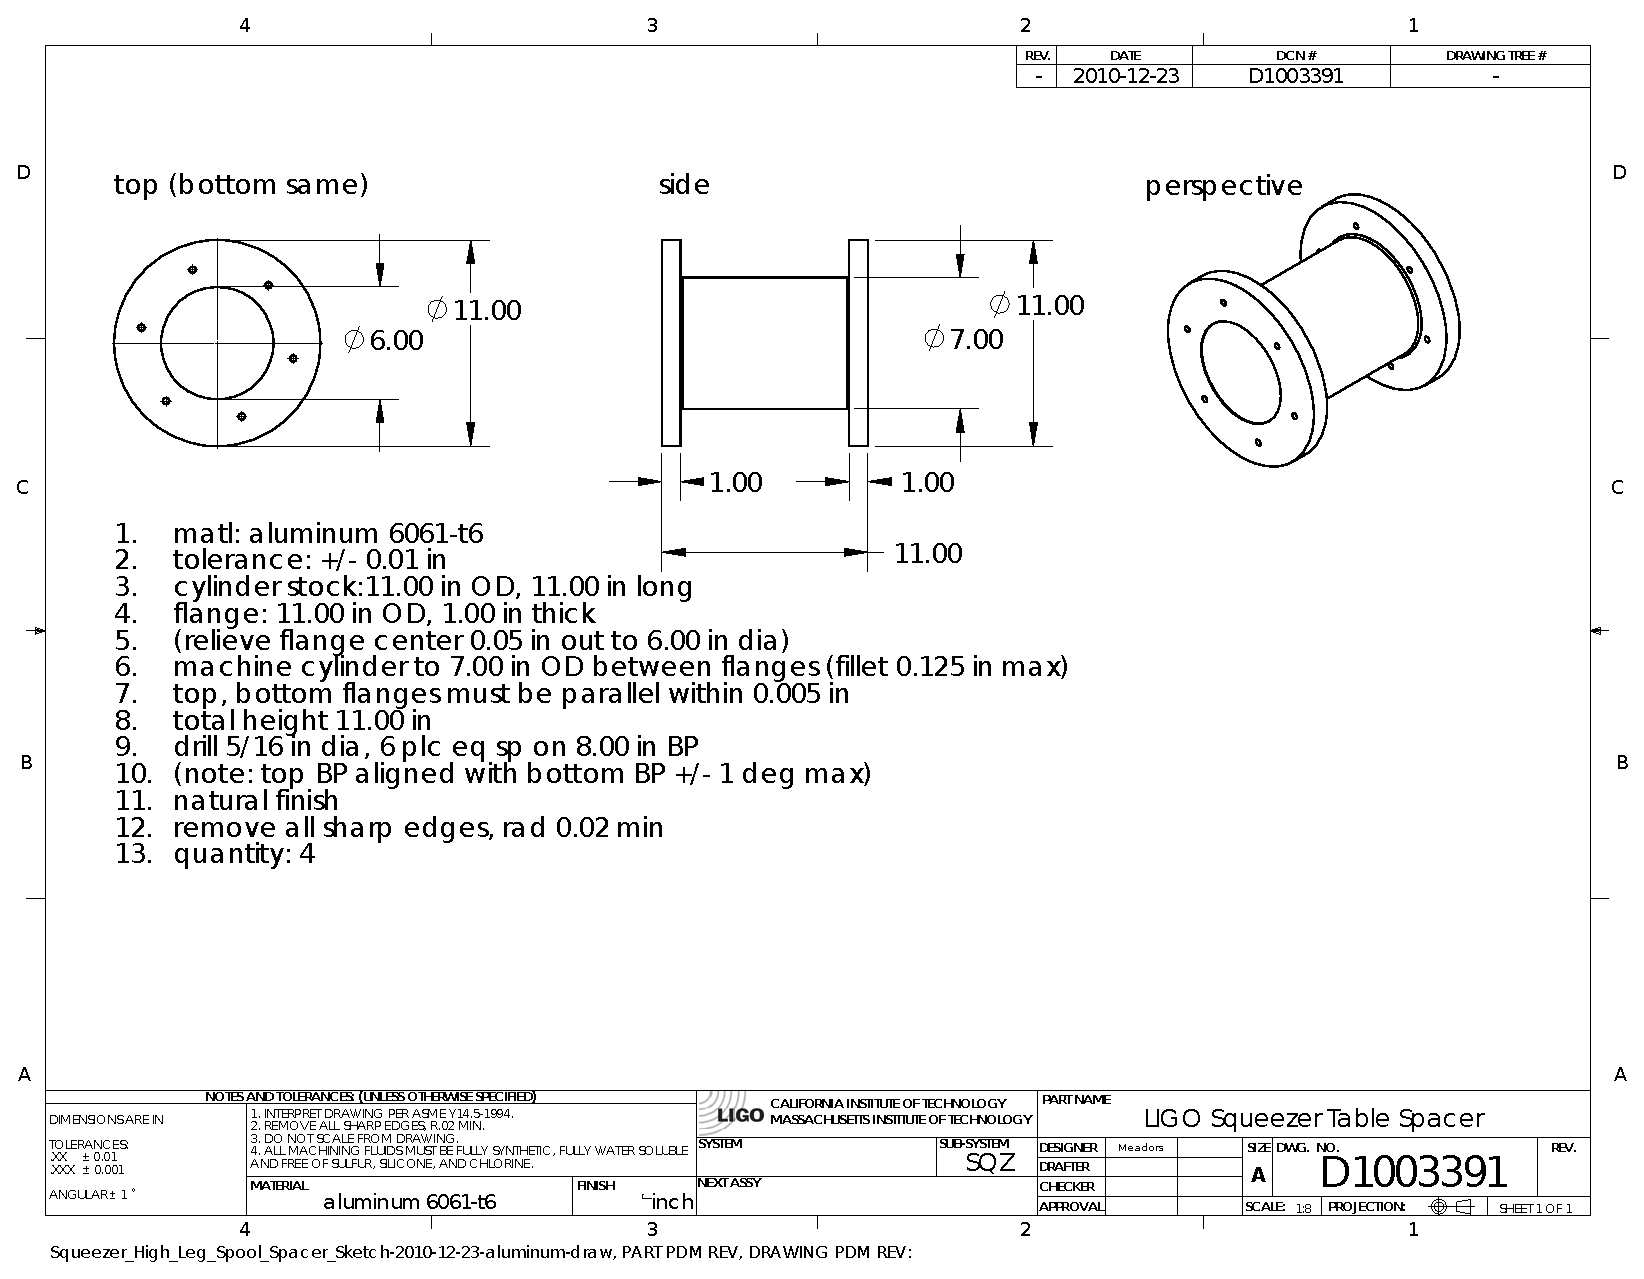
\includegraphics[width=0.6\paperwidth]{Squeezer_High_Leg_Spool_Spacer_2010-12-23_aluminum.eps}
\caption{Table legs SolidWorks schematic. This initial design for the table leg extensions on the squeezer table incorporated a flange, which was removed immediately prior to fabrication, replaced with a larger diameter flangeless tube with incorporated tap-holes. Flanges were thought necessary for a flexible alignment initially, they would be prohibitively expensive to machine, and welding would induce unacceptable distortions into the metal. Design in consultation with Daniel Sigg, Lisa Barsotti, Keita Kawabe, Gerardo Moreno, Richard Savage.
}
\label{spacer_legs_figure}
\end{center}
\end{figure}


            \subsubsection{Faraday isolator measurement}
            \label{Faraday}

                %Faraday isolator measurements were performed by Keita Kawabe, Matt Evans, Lisa Barsotti along with myself.

		%What were the results of the measurement? Show e-log entries, comment on in-and-out-of-vacuum performance and what it says about the need for low loss to be a top priority in future squeezing efforts.

Squeezing is helpful only if helps detector sensitivity more than harms it.
Backscattered light from the interferometer, reflected by the squeezer back into the main detector~\cite{ChuaThesis,BarsottiNatureSqueezing}, is a serious concern, particularly phase noise in the scattered light fields.
In order to mitigate this, an additional Faraday isolator is put into the optical path of the squeeze beam, which acts to supplement the intrinsic 40 dB isolation thanks to the OPO.
Measuring the isolation ratio of this Faraday isolator was a task for Kawabe, Barsotti, Evans, and myself.

Our results \footnote{See \url{http://ilog.ligo-wa.caltech.edu/ilog/pub/ilog.cgi?group=detector&date_to_view=06/09/2011&anchor_to_scroll_to=2011:06:09:16:58:36-lisabar} for more details.} were that Faraday isolator, as measured in air, transmitted 480 of 500 mW injected in the correct direction (96\% transmission), attenuated 460 mW to 35 $\mu$W when injected in the wrong direction (-41.3 dB isolation ratio), and would back-scatter 2.5 mW of 500 mW (-23 dB) input power toward the squeezer. 
These numbers sufficed to proceed with in-vacuum installation.

            \subsubsection{In-vacuum installation}
            \label{In-vacuum}

Installing the the additionally Faraday isolation in vacuum was necessary before the squeezed beam from the table could be injected directly into the dark port.
The new Faraday, but not the existing initial LIGO Faraday, had an opening to accommodate the beam. 
Because Advanced LIGO installation, concurrent with the squeezing experiment, involved opening the vacuum, our own installation (Kawabe, Barsotti, Dwyer, Chua, Gustafson, and the author) were able to emplace and align the new Faraday isolation on the optical table inside HAM4, move a baffle in HAM5 (optically downstream), and direct the beam onto HAM6 (the optical terminus), the location of the output photodiode\footnote{Detailed in \url{http://ilog.ligo-wa.caltech.edu/ilog/pub/ilog.cgi?group=detector&date_to_view=06/29/2011&anchor_to_scroll_to=2011:06:29:18:31:51-lisabar} on the electronic log.}.
                %In-vacuum Faraday and baffle installation with "".
                %Show pictures of the installation, connect to the issues with stray and perhaps backscattered light.

Once the squeezing beam was on the output photodiode, the vacuum enclosure pumped down and H1 restored to operation,
\footnote{And local wildlife rescued: \url{http://ilog.ligo-wa.caltech.edu/ilog/pub/ilog.cgi?group=detector&date_to_view=09/23/2011&anchor_to_scroll_to=2011:09:23:21:37:25-sheilad}}, 
it was determined that the interferometer was not functioning as expected.
The output mode cleaner transmission was about 25\% lower than previously measured~\cite{Waldman2011,SmithThesis}.
This loss was severe enough to warrant an additional vacuum incursion.
Our task was to install the now-unused L1 OMC as a tentative replacement. 
First, Evans, Barsotti, Chua, Kawabe and myself verified\footnote{See \url{http://ilog.ligo-wa.caltech.edu/ilog/pub/ilog.cgi?group=detector&date_to_view=10/21/2011&anchor_to_scroll_to=2011:10:21:11:12:21-sheon}} that the L1 OMC had superior finesse to that inferred for the H1 OMC.
A rapid replacement of the H1 OMC by the L1 followed, over the course of two days\footnote{Day 1: \url{http://ilog.ligo-wa.caltech.edu/ilog/pub/ilog.cgi?group=detector&date_to_view=10/24/2011&anchor_to_scroll_to=2011:10:25:09:11:32-kawabe} \\ Day 2: \url{http://ilog.ligo-wa.caltech.edu/ilog/pub/ilog.cgi?group=detector&date_to_view=10/25/2011&anchor_to_scroll_to=2011:10:25:19:49:56-kawabe}},
involving Bram Slagmolen, Smith-Lefebvre, Kawabe, Evans, Dwyer, Chua, Factourovich and myself.
Once installation was complete and the vacuum pumped down, H1 returned to operation.

In the optics lab, the H1 OMC was found~\cite{Waldman2011} to have one of its control elements, a heater, out of place. 
It was occulting the beam inside its resonant bowtie cavity, reducing the finesse.
In any event, the transplanted L1 OMC worked as intended inside H1.

%		Discuss the repair of the output mode cleaner, which is mentioned (citation 50) in Nic's thesis~\cite{SmithThesis}. 
%The technical report corresponding to it is by Waldman and Chua~\cite{Waldman2011}.

            \subsubsection{Data digitization}
            \label{data_digitization}

Full control of the squeezer required more of its digital computer input and readout to be accessible proximal to the rest of the interferometer controls.
Ere H1 was resuscitated, the author made and helped lay cables and, with Dave Barker, selected computer channels for the analog-to-digital conversion of squeezer data \footnote{Fuller information in the electronic log: \url{http://ilog.ligo-wa.caltech.edu/ilog/pub/ilog.cgi?group=detector&date_to_view=08/16/2011&anchor_to_scroll_to=2011:08:16:21:27:49-gmeadors} and \\ \url{wa.caltech.edu/ilog/pub/ilog.cgi?group=detector&date_to_view=08/26/2011&anchor_to_scroll_to=2011:08:26:15:08:16-gmeadors}}.
Measurements began.

                %Electronic cabling and analog-to-digital converter installation.
                %Added data channels with David Barker.


		%May want helpful diagram.

%\end{frame}

%\begin{frame}{Squeezing large interferometers}



%\end{frame}

%\begin{frame}{Squeezing's scientific benefit}
\subsection{Squeezing's scientific benefit}

Squeezing worked in spite of optical losses, did not make the interferometer worse, and in fact increased shot noise limited performance by over 2 dB~\cite{BarsottiNatureSqueezing}.
The benefits translate directly into measurement scientific benefits.

\begin{figure}
\begin{center}
%\protect\caption{\protect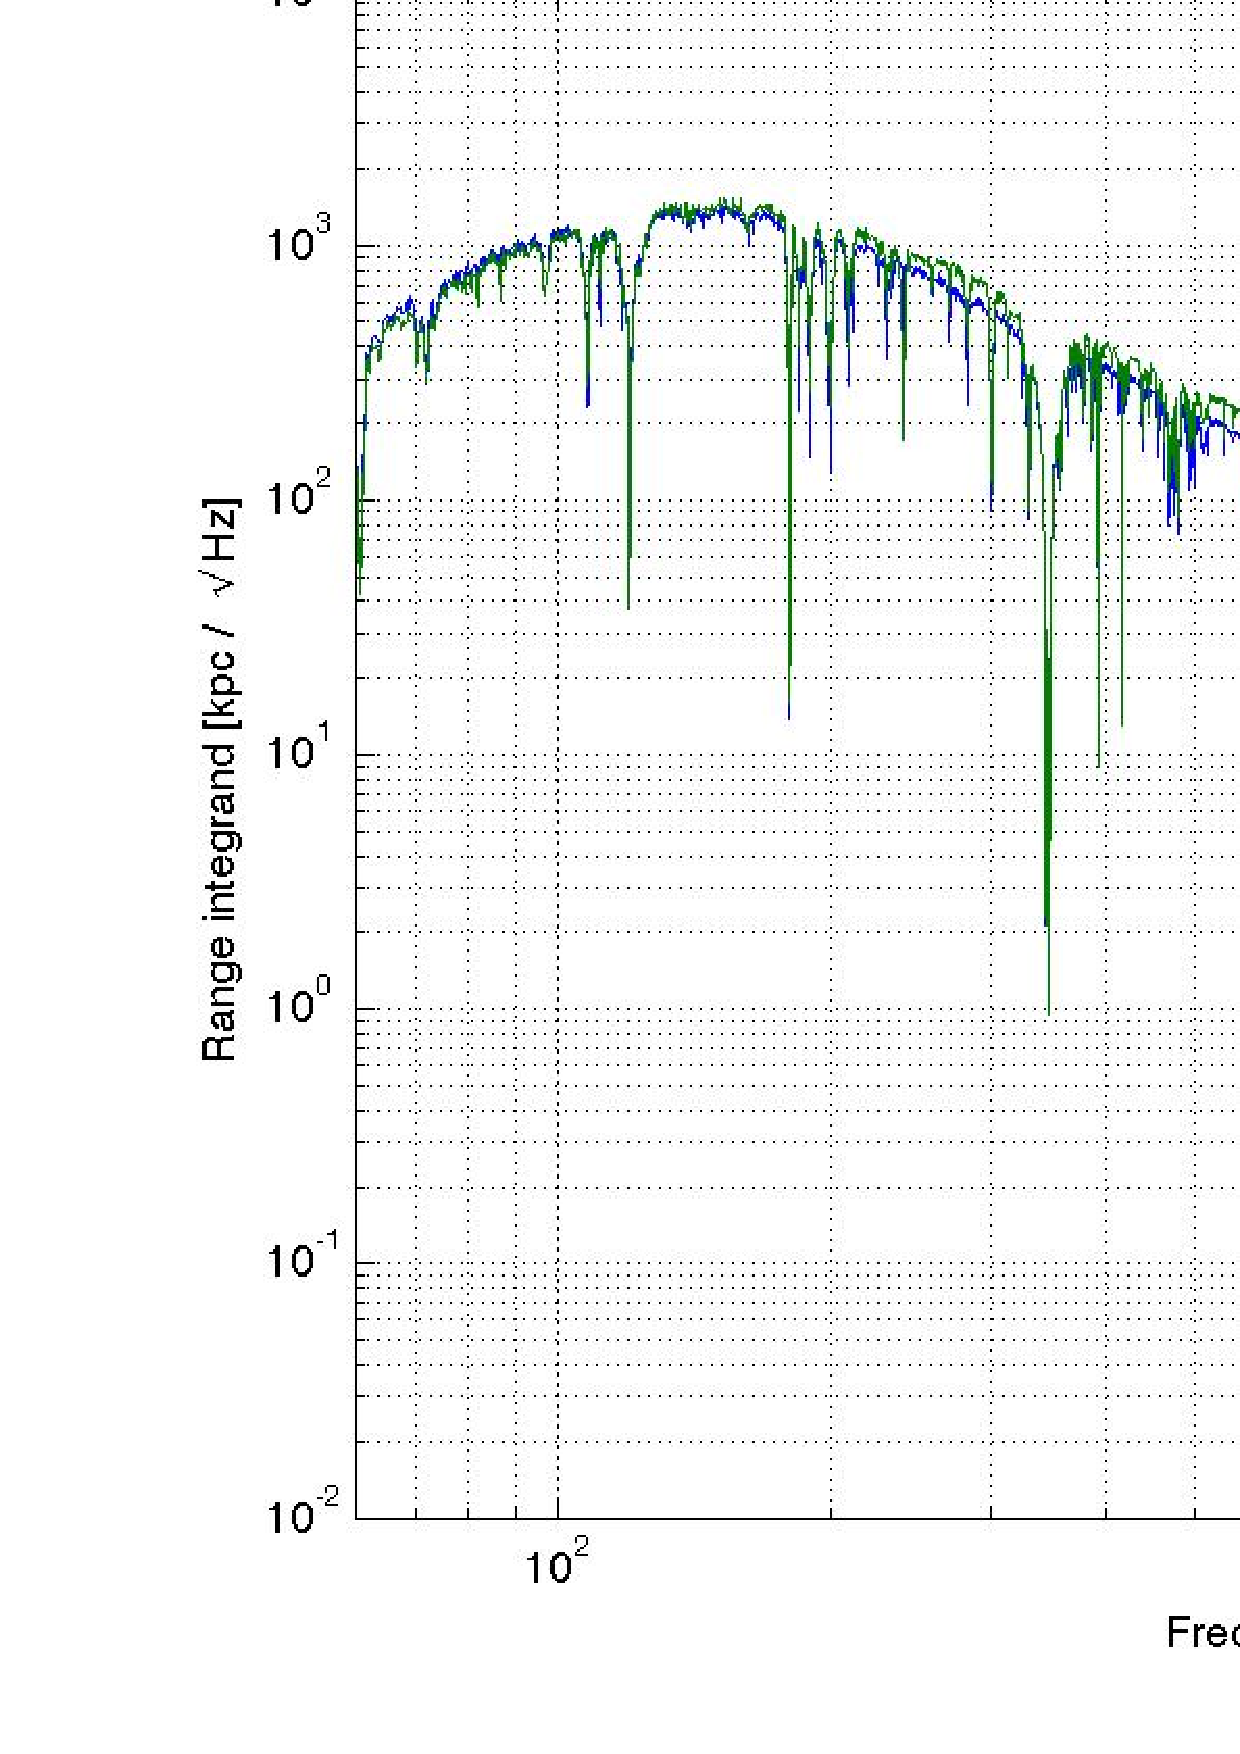
\includegraphics[width=0.45\paperwidth,height=0.45\paperheight,keepaspectratio]{range_integrand.jpeg}\protect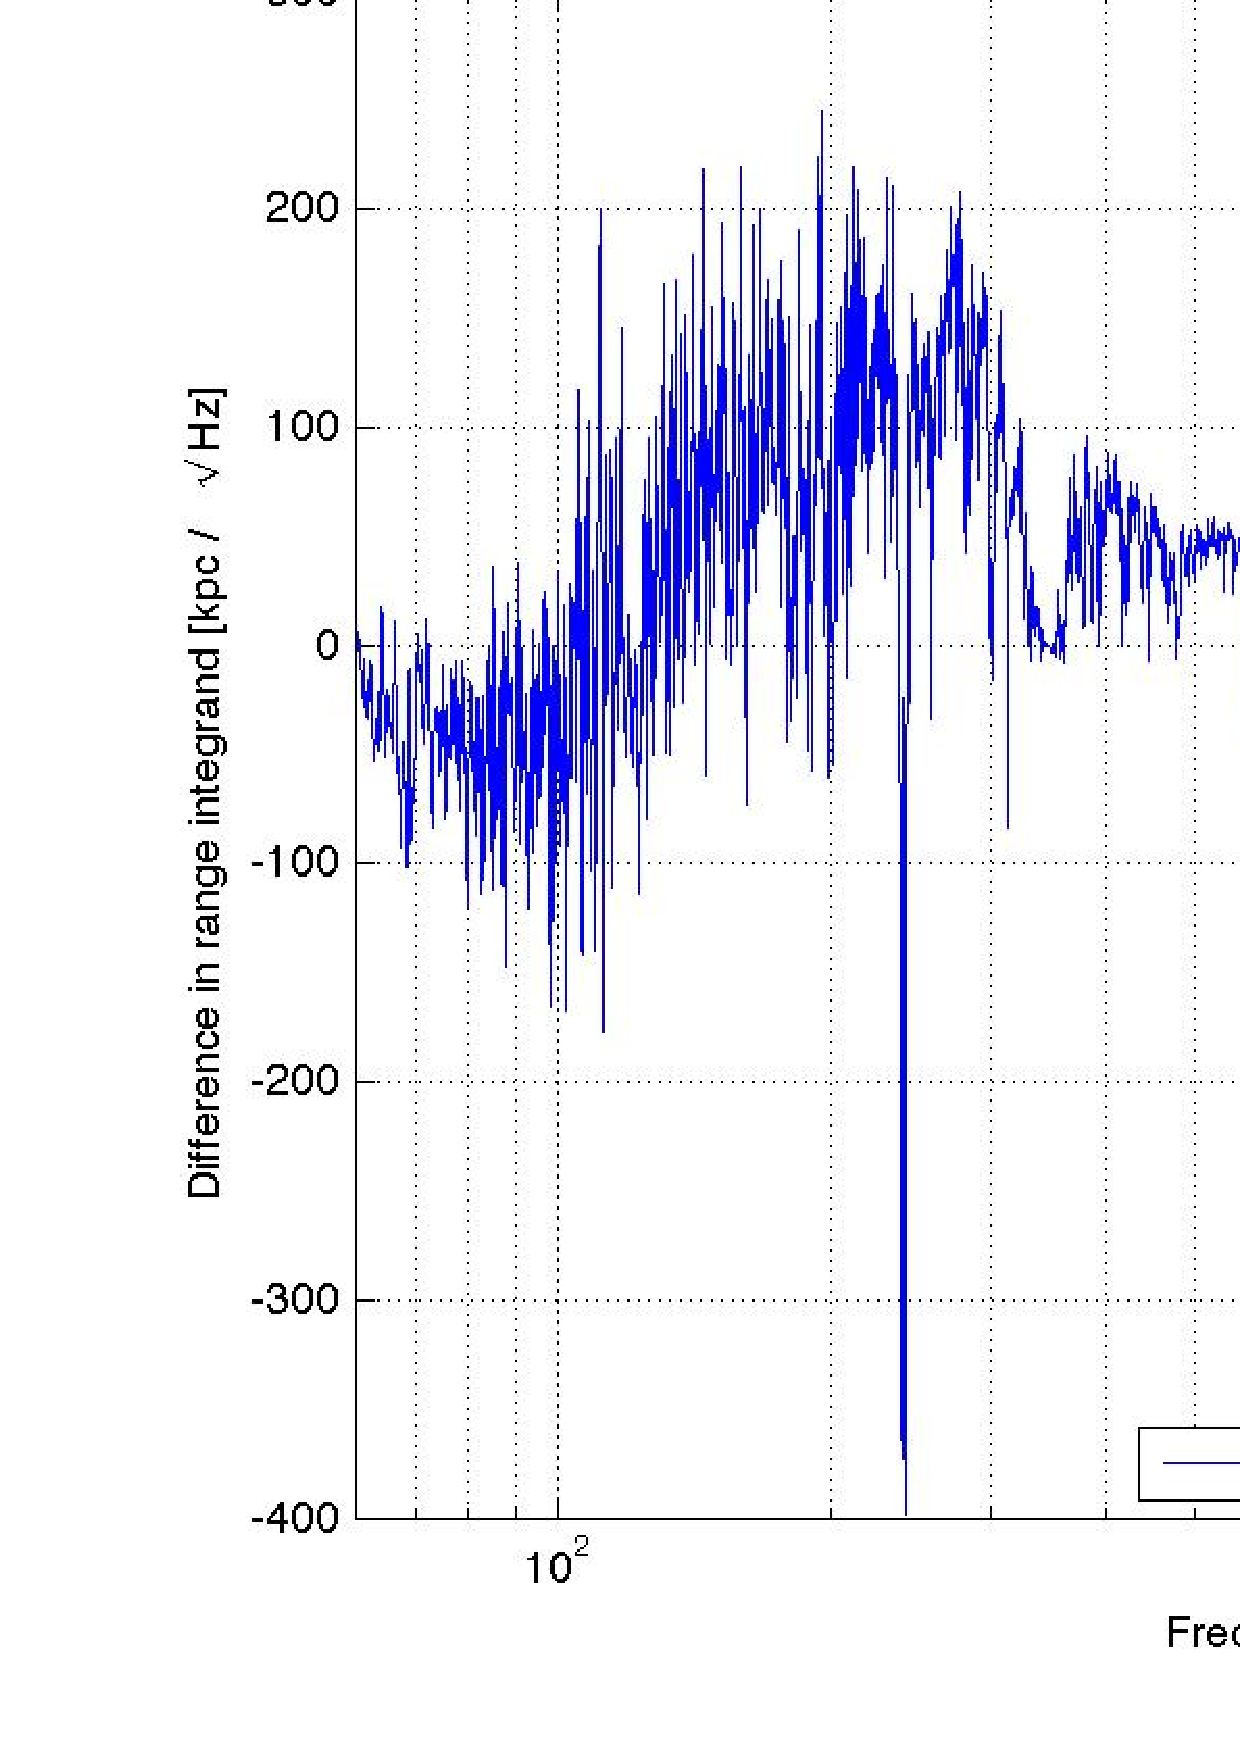
\includegraphics[width=0.45\paperwidth,height=0.45\paperheight,keepaspectratio]{range_integrand_difference.jpeg}}
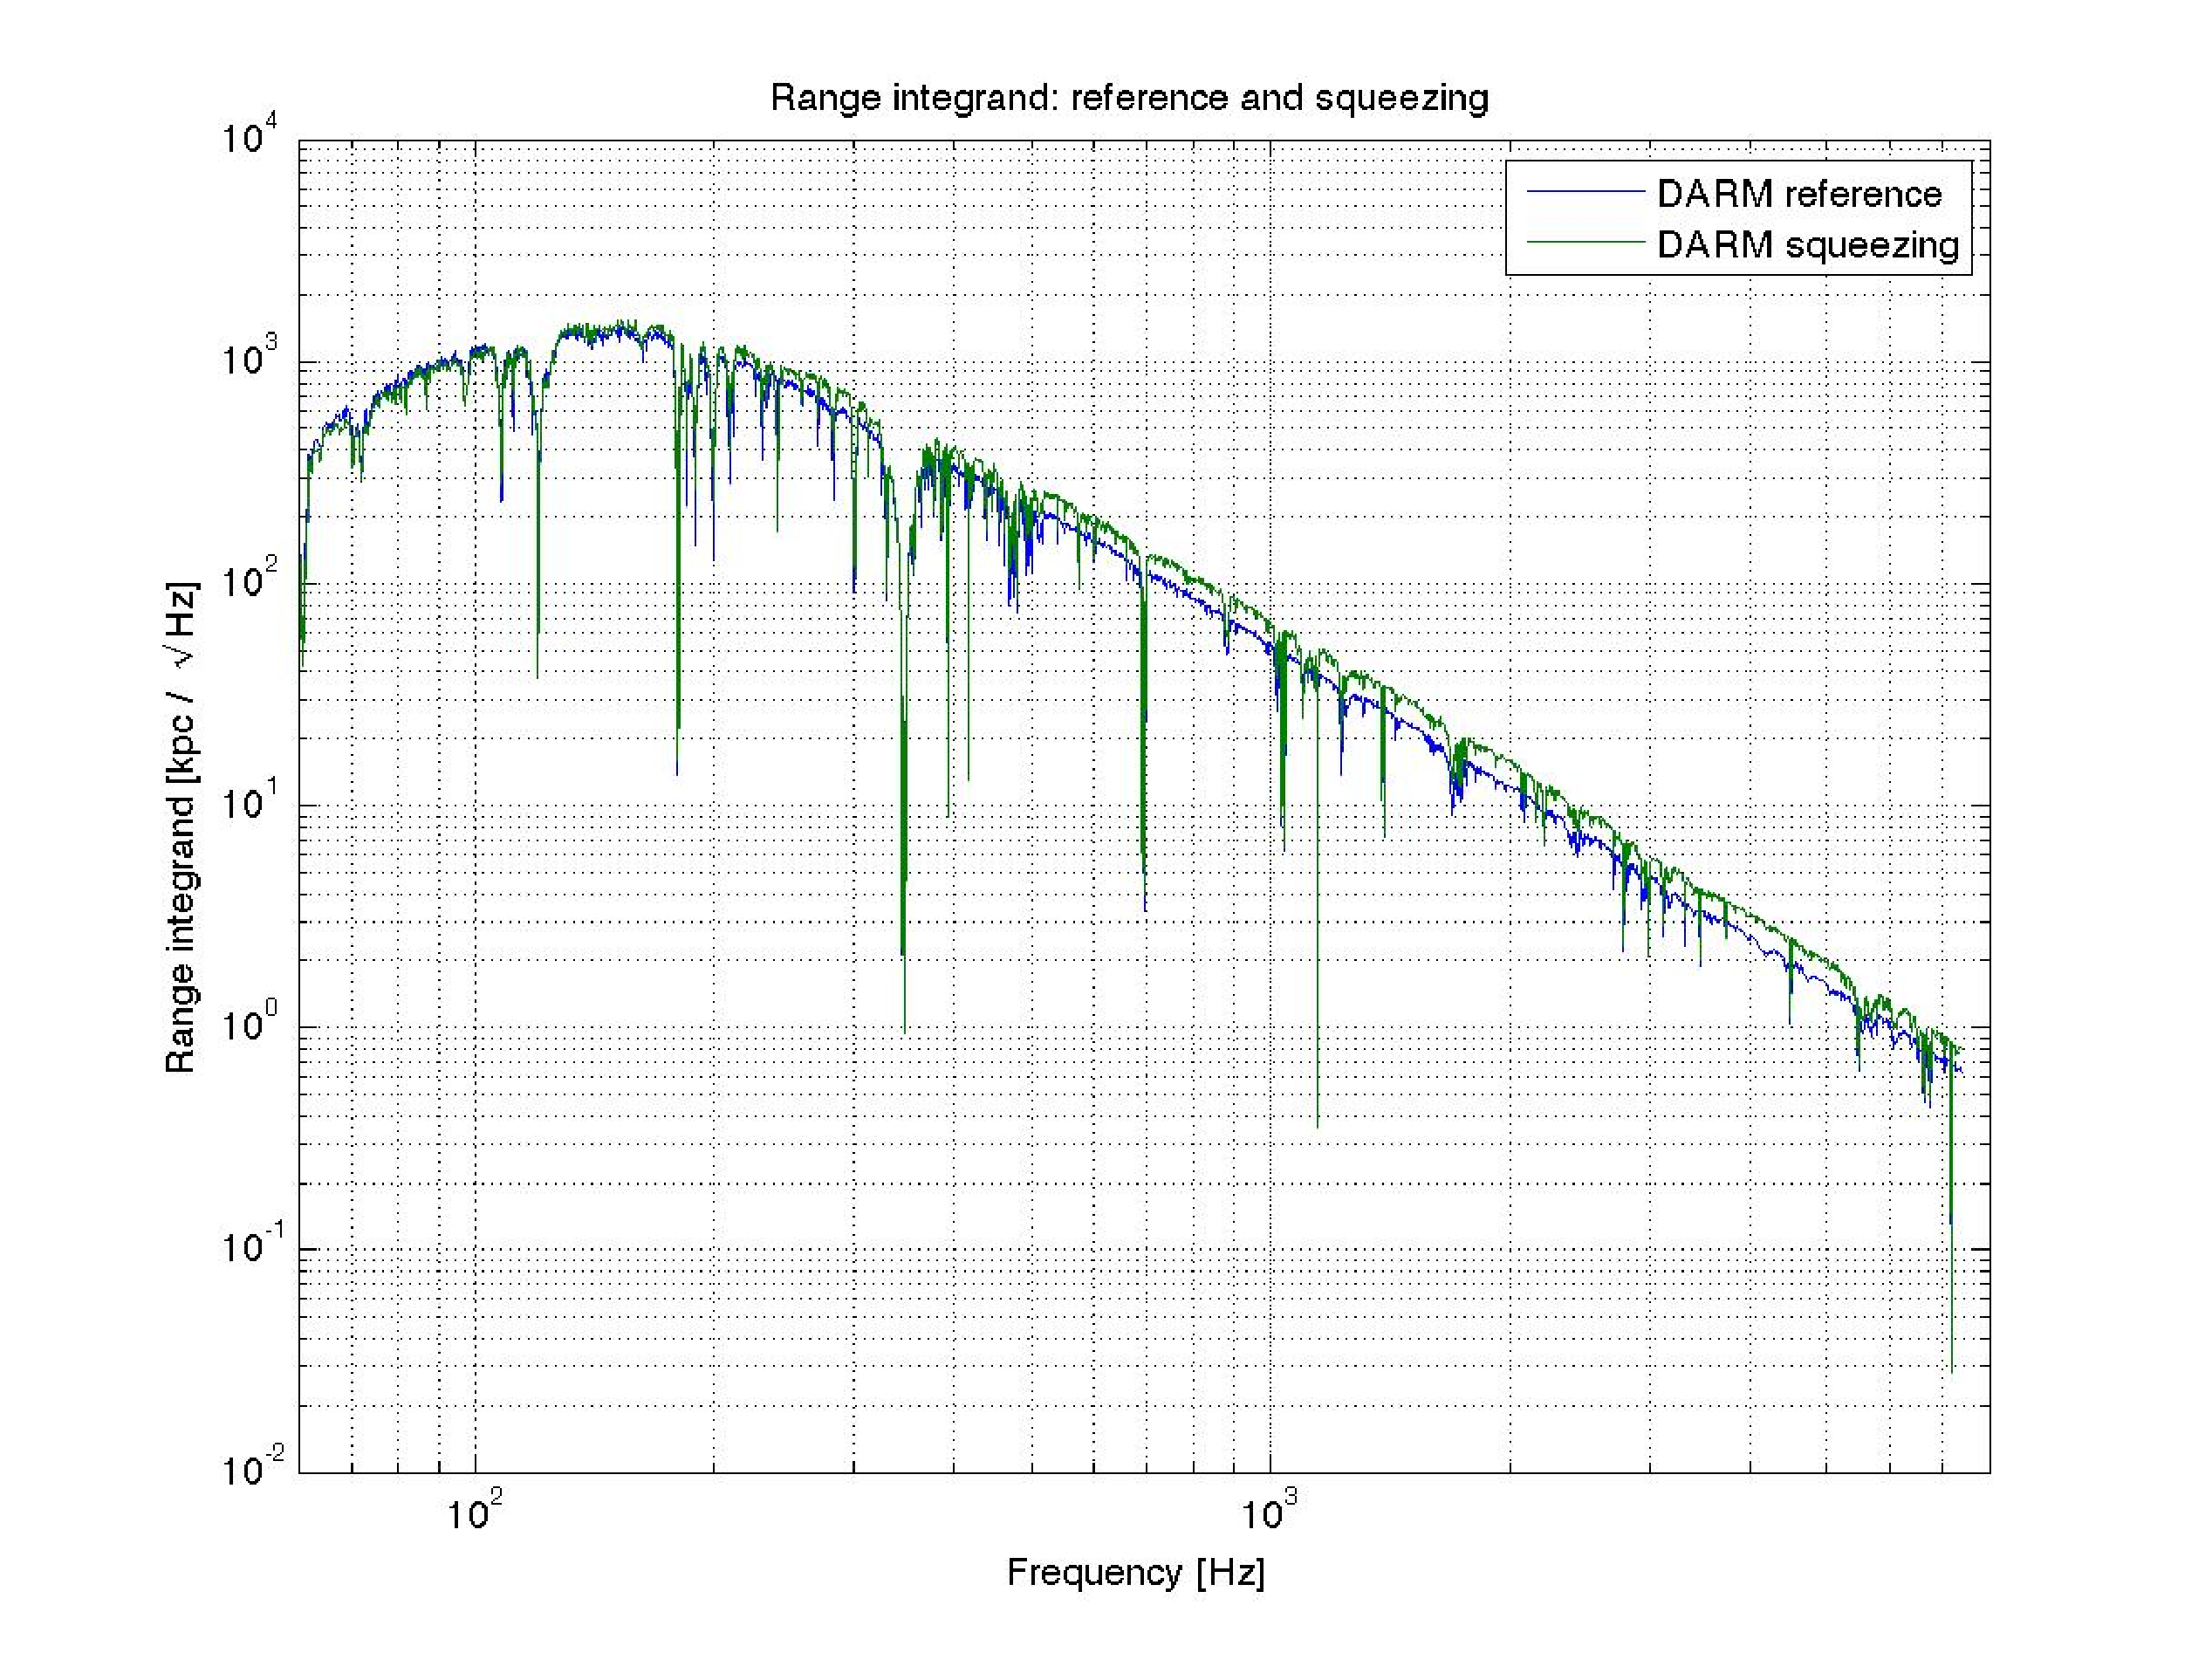
\includegraphics[height=0.5\paperheight, width=0.5\paperwidth,keepaspectratio]{range_integrand.eps}
\caption{Integrand of inspiral range as a function of frequency, with and without squeezing.}
\label{squeezing_range_integrand}
\end{center}
\end{figure}

\begin{figure}
\begin{center}
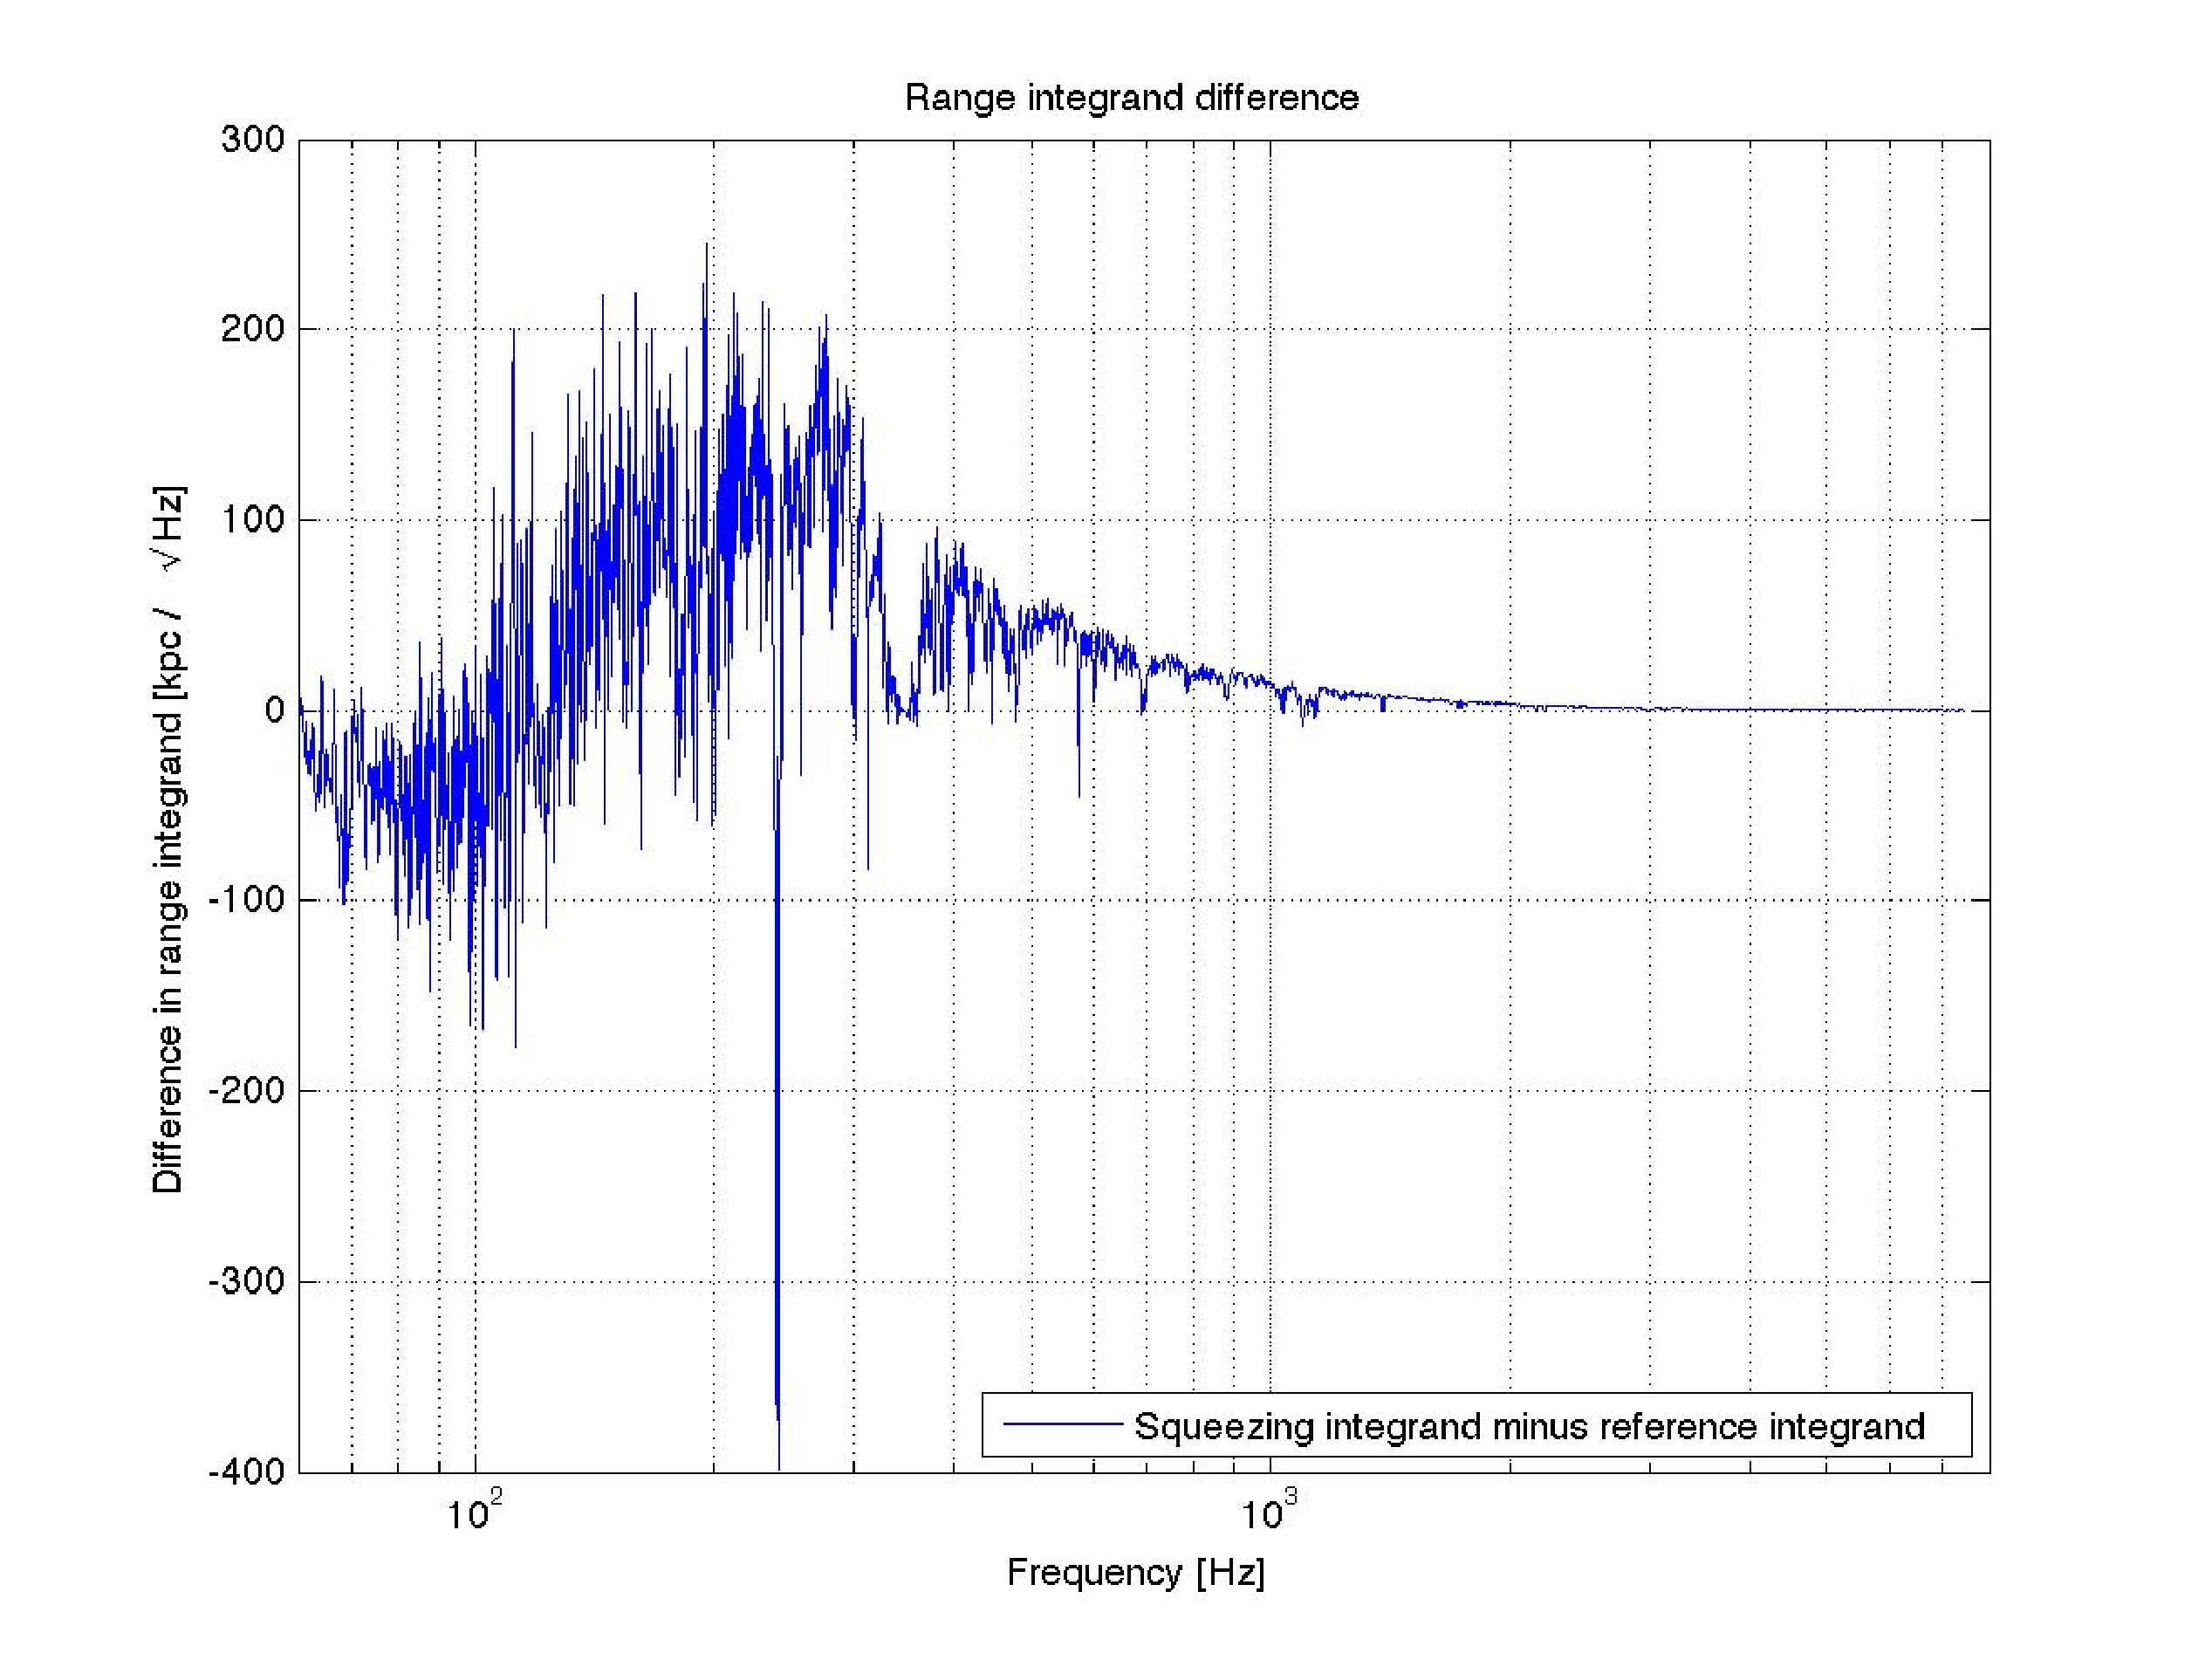
\includegraphics[height=0.5\paperheight, width=0.5\paperwidth,keepaspectratio]{range_integrand_difference.eps}
\caption{Net effect of squeezing on inspiral range integrand. Scientific benefit from squeezing is evident at the few hundred Hz `bucket' where initial LIGO is most sensitive, and although low frequency noise is slightly worse, this in an already noisy spectral band. Enhanced LIGO unambigiously benefitted from squeezing, proving the technique's efficacy.
}
\label{squeezing_range_net}
\end{center}
\end{figure}

            \subsubsection{Figures of merit: inspiral range}
            \label{range_est}
                %Range estimation after squeezing

As noted in Chapter~\ref{chap3}, gravitational wave interferometers are regularly characterized by their inspiral range~\cite{FinnInspiral1993}.
This figure of merit integrates the gravitational wave strain spectrum into a single number: the distance to which a pair of 1.4 solar mass neutron stars (canonically, with average orientation and sky location and a signal-to-noise ratio of 8, although definitions differ) could be detected if they inspiralled together:

\begin{equation}
F_{7/3} = \int_{f_l}^{f_h} \left[f^{7/3} h^2(f) \right] df,
\label{f-seven-thirds-squeezing}
\end{equation}
\begin{equation}
R = \Theta \left( \frac{5 c^{1/3} M_\textup{ch}^{5/3} F_{7/3}}{96 \pi^{4/3} \textup{SNR}_0} \right)^{1/2} L,
\label{inspiral_range_squeezing}
\end{equation}

\noindent where R is inspiral range in kiloparsec, $f$ is frequency, $h$ the strain sensitivity as a function of frequency, $\Theta$ is a correction factor of $1.77$ for orientation and sky location, $c$ is the speed of light, $M_\textup{ch} = G c^{-2} M_\textup{sun} (M_1 M_2)^{3/5} (M_1+M_2)^{-1/5}$ is the chirp mass of two stars with masses $M_1 = M_2 = 1.4 M_\textup{sun}$, $F_{7/3}$ is as defined in Equation~\ref{f-seven-thirds-squeezing}, $\textup{SNR}_0$ is typically 8, and $L$ is the interferometer length in meters.
The range integrand in Equation~\ref{f-seven-thirds-squeezing} can itself be multiplied by the external coefficients in Equation~\ref{inspiral_range_squeezing} to yield a plot of the contribution of each frequency band to the scientific performance of the interferometer, as in Figure~\ref{squeezing_range_integrand}.
Taking the difference of before- and after-squeezing shows where squeezing yielded improvement -- and demonstrates that it did not seriously degrade interferometer performance\footnote{For additional plots in the log, \url{http://ilog.ligo-wa.caltech.edu/ilog/pub/ilog.cgi?group=detector&date_to_view=11/30/2011&anchor_to_scroll_to=2011:11:30:12:54:18-gmeadors}\\feedforward MICH correction was attempted but unneeded, as detailed also, \url{http://ilog.ligo-wa.caltech.edu/ilog/pub/ilog.cgi?group=detector&date_to_view=12/02/2011&anchor_to_scroll_to=2011:12:02:15:06:38-gmeadors}.}.

		From the improved high frequency shot noise, we can see that squeezing bought Enhanced LIGO a megaparsec of inspiral range. 
This number is impressive in several respects: our goal was to acheive a squeezing factor of perhaps as much as 3 dB, but to do it in the shot noise-limited region, at high frequencies, where the inspiral range equations 
 count for much less. 
%(MATH: add the inspiral range equation if not already shown for feedforward!)
The range integrand shows squeezing down to 150 Hz, which is the lowest yet achieved for a gravitational wave interferometer, as can be seen in the Nature Photonics paper~\cite{BarsottiNatureSqueezing}.
Squeezing such low frequencies brings most of the inspiral range improvement.
In all, the squeezer experiment added about another five percent to H1's range, but also something more significant: prospects for enhancing gravitational wave interferometers beyond the standard quantum limit. 

\section{Squeezing large interferometers: success and prospects}
\label{squeezing_success}

        %\subsection{Success and Advanced LIGO prospects}
            %Results and hopes for aLIGO+ squeezing.

	    Over 2 dB of squeezing were achieved by the LIGO Hanford squeezing experiment on H1~\cite{BarsottiNatureSqueezing}. Building on the previous success of GEO600~\cite{GEO600NatureSqueezing}, squeezing is now a mature technique that we hope to incorporate into LIGO permanantly as soon as it is feasible.
Publications by Dwyer~\cite{DwyerPhaseNoise} and Chua~\cite{ChuaBackscatteredLight} detail the remaining hurdles.
Dwyer notes that quadrature phase noise will become increasingly significant as losses are reduced, particularly for filter cavities.
Chua proposes a path toward reduced backscattered light noise.
% since I am an author on both of them. We have a preliminary understanding now of at least two major problems: the quadrature phase noise fluctatuations and backscattered light. Backscattered light can be resolved in several ways. Phase noise must be progressively improved, as Sheila discusses, because we can hope to acheive the mature filter cavity design proposed below.
As we develop an understanding of these two principal problems, work at MIT is progressing (led by Tomoki Isogai) on realizing a filter cavity suitable for the LIGO frequency band.
With it, future interferometers will be able to introduce frequency-dependent squeezing to finally reduce, not just shot noise, but radiation pressure as well, below the standard quantum limit.
If all else works, gravitational wave interferometers may soon be able to detect a wide variety of astrophysically interesting sources.

%Discuss Lisa Barsotti's talk about the future prospect for LIGO using filter cavities, work that Tomoki Isogai is doing. With filter cavities, we can acheive frequency-dependent squeezing, having the best of both works by reducing quantum radiation pressure noise at low frequencies and shot noise at high, by using the filter cavity to produce a squeezed vacuum with a squeeze angle that varies as a function of frequency. Though as yet this filter cavity has yet to be constructed, it is in the works at MIT.

% Everything below is imported from my AEI talk

%\end{frame}

%\begin{frame}{Squeezing summary}
%\subsection{Squeezing summary}

%\begin{description}
%\item [{Instrumental}] experience with technique important beyond Advanced
%LIGO
%\item [{Physical}] way to improve broad band of LIGO, benefit many searches
%\item [{Illustrates}] need for best sensitivity at few hundred Hz
%\item [{Question}] what can we improve \emph{post-facto?}
%\end{description}
%\end{frame}


%        -------------------------------- 
%
%	The following is an example of using the commands \textit{ref}
%	and \textit{label}. With these commands theorems, chapters,
%	sections and figurres can be labeld with names in the tex file
%	and then refered to by these names in later tex files. In
%	chapter~\ref{intro} we saw section~\ref{sample_section} or
%	theorem~\ref{sample_theorem}.
%
%	Lastly, here is how to include a figure. First generate an
%	encapsulated postscript file in xfig, adobe illustrator or
%	some other program. The specific commands are found in
%	\textit{chap2.tex}.
%
%        \begin{figure}[htb]
%        \centerline{ \epsfig{figure=sample.eps, 
%        height =  1.5 in}}
%        \caption{Sample Figure}
%        \label{sample_figure}
%        \end{figure}

